% =============================================
% ==       sections/experiments.tex          ==
% =============================================
\section{Experiments}\label{sec:experiments}

This section presents our experimental setup, evaluation metrics, and results. We compare our method with several baselines.

This experiment aims to systematically and comprehensively compare the performance of four algorithms in the field of multi-agent deep reinforcement learning—namely, MAPPO, QMIX, OW-QMIX, and IPPO—across various StarCraft maps with different environmental configurations. The results are intended to provide a scientific and reliable experimental basis and theoretical support for algorithm selection and optimization in complex, dynamic game environments within multi-agent systems.

\subsection{Experimental Setup}
\subsubsection{Environment}

StarCraft II serves as the core experimental platform in this study. It is chosen for its sophisticated multi-agent interaction dynamics, real-time adversarial challenges, and extensive unit control capabilities, which collectively create an ideal and congruent simulation environment for assessing multi-agent reinforcement learning algorithms.

Based on the experimental objective of comparing the performance of the four algorithms under scenarios with varying coordination demands and unit configurations, this experiment selects two maps with typical differences: \texttt{1m\_vs\_2z} and \texttt{5m\_vs\_6m}. 

\paragraph{Map \texttt{1m\_vs\_2z}} 
Our side consists of 1 ``Marine'' (abbreviated as \texttt{m}), while the enemy consists of 2 ``Zerglings'' (abbreviated as \texttt{z}). This unit matchup fully aligns with the adversarial relationship defined by the env\_id. The map lacks complex terrain obstacles, eliminating environmental interference with unit coordination and allowing the experiment to focus more on the agents' decision-making logic.

The mission objective is clear and straightforward: eliminate the enemy unit through coordination between the agents while ensuring the survival of our Marines as much as possible. The mission is deemed a failure if all our units are eliminated or if the enemy remains alive for too long. This setup not only aligns with the core mechanics of StarCraft II but also highly suits the experimental goal of testing coordinated decision-making in multi-agent algorithms. It effectively evaluates the algorithms' ability to balance the trade-off between ``attacking'' and ``surviving''.

\paragraph{Map \texttt{5m\_vs\_6m}} 
This map represents a classic scenario centered on coordinated combat under numerical disadvantage, with its design focused on testing multi-agent collaboration capabilities among homogeneous units. Our side controls a team of Marines, while the enemy consists of a larger group of Marines. Both sides use identical unit types, eliminating any rock-paper-scissors-type advantages and shifting the core challenge entirely to multi-agent coordination and tactical execution.

The battlefield is more expansive compared to basic maps, providing ample space for multi-unit positioning and formation adjustments. In terms of initial deployment, our units are arranged in a linear formation, while the enemy units are distributed in a fan-shaped encirclement, creating a naturally tactically oppressive setup. This configuration requires the agents to actively adjust formations and optimize attack priorities to break the passive situation.

The map contains no terrain obstacles, further simplifying environmental variables and allowing the experiment to precisely focus on the agents' target assignment and action synchronization capabilities. During dynamic engagements, agents must continuously assess the threat level of enemy units. The mission fails if all allied units are eliminated or if the combat duration exceeds the time limit.

\subsubsection{Evaluation Metrics}
We assess the performance of each algorithm based on three primary metrics:
\begin{itemize}
    \item \textbf{Allies-Dead-Ratio:} To reflect the proportion of allied agents lost during training, used to track the algorithm's learning progress in developing protective strategies for friendly units throughout the training process.
    \item \textbf{Enemies-Dead-Ratio:} To reflect the proportion of enemy agents eliminated during training, used to monitor the algorithm's learning progress in developing effective enemy neutralization strategies during the training period.
    \item \textbf{Win-Rate:} To indicate the probability of the algorithm successfully completing missions during training, used to track the improvement in the algorithm's mission accomplishment capability throughout the training process.
\end{itemize}

\subsubsection{Implementation Details}
\paragraph{Codebase Used}
The experiment employs XuanCe (\urlstyle{tt}\url{https://github.com/agi-brain/xuance}) as the\\ core codebase~\cite{liuXuanCeComprehensiveUnified2023}.\@
It specializes in reinforcement learning and multi-agent systems research, demonstrating exceptional performance in algorithm development for complex multi-agent environments such as StarCraft II.
For instance, by utilizing the $\texttt{xuance.environment.make\_envs}$ function, multi-agent interaction scenarios like \texttt{1m\_vs\_2z} and \texttt{5m\_vs\_6m} can be directly created. The framework automatically handles underlying tasks such as unit state observation extraction, available action parsing, and reward signal generation, eliminating the need for manual implementation of interaction logic with StarCraft II.
This significantly simplifies and streamlines the environment setup process, enabling faster experimental testing.

\paragraph{Hyperparameter Settings}
We list the respective key parameters of the two maps in table~\ref{tab:hyperparameters_detailed}.
\begin{table*}[ht]
\centering
\caption{Detailed hyperparameter settings for the SMAC maps.}%
\label{tab:hyperparameters_detailed}
\begin{tabular}{lcc}
\toprule
\textbf{Hyperparameter} & \textbf{2m\_vs\_1z} & \textbf{5m\_vs\_6m} \\
\midrule
Learning Rate & 0.0007 & 0.0007 \\
Batch Size & 128 & 128 \\
Network Architecture & GRU (64-dim) + 3$\times$64 MLP & GRU (64-dim) + 1$\times$64 MLP \\
Discount Factor ($\gamma$) & 0.99 & 0.99 \\
GAE Coefficient ($\lambda$) & 0.95 & 0.95 \\
PPO Clipping Coeff. ($\epsilon$) & 0.2 & 0.05 \\
Total Training Steps & 1,000,000 & 10,000,000 \\
Random Seed & 1 & 1 \\
Computing Device & \texttt{cuda:0} & \texttt{cuda:0} \\
\bottomrule
\end{tabular}
\end{table*}

\subsection{Experiments and Results}\label{sec:results}
In this section, we present the empirical results of our comparative study. We systematically evaluate the performance of MAPPO, QMIX, OW-QMIX, and IPPO across various SMAC scenarios. We begin by analyzing a representative easy map with homogeneous agents to establish a baseline understanding of the algorithms' core performance characteristics.

\subsubsection{Map \texttt{1m\_vs\_2z}}
We first evaluate the algorithms on the \texttt{1m\_vs\_2z} map.The performance of the four algorithms is visualized in Figure~\ref{fig:results_1m_vs_2z}, with final quantitative results summarized in Table~\ref{tab:results_1m_vs_2z}.

\begin{figure*}[ht!]
    \centering
    \begin{subfigure}[b]{0.32\textwidth}
        \centering
        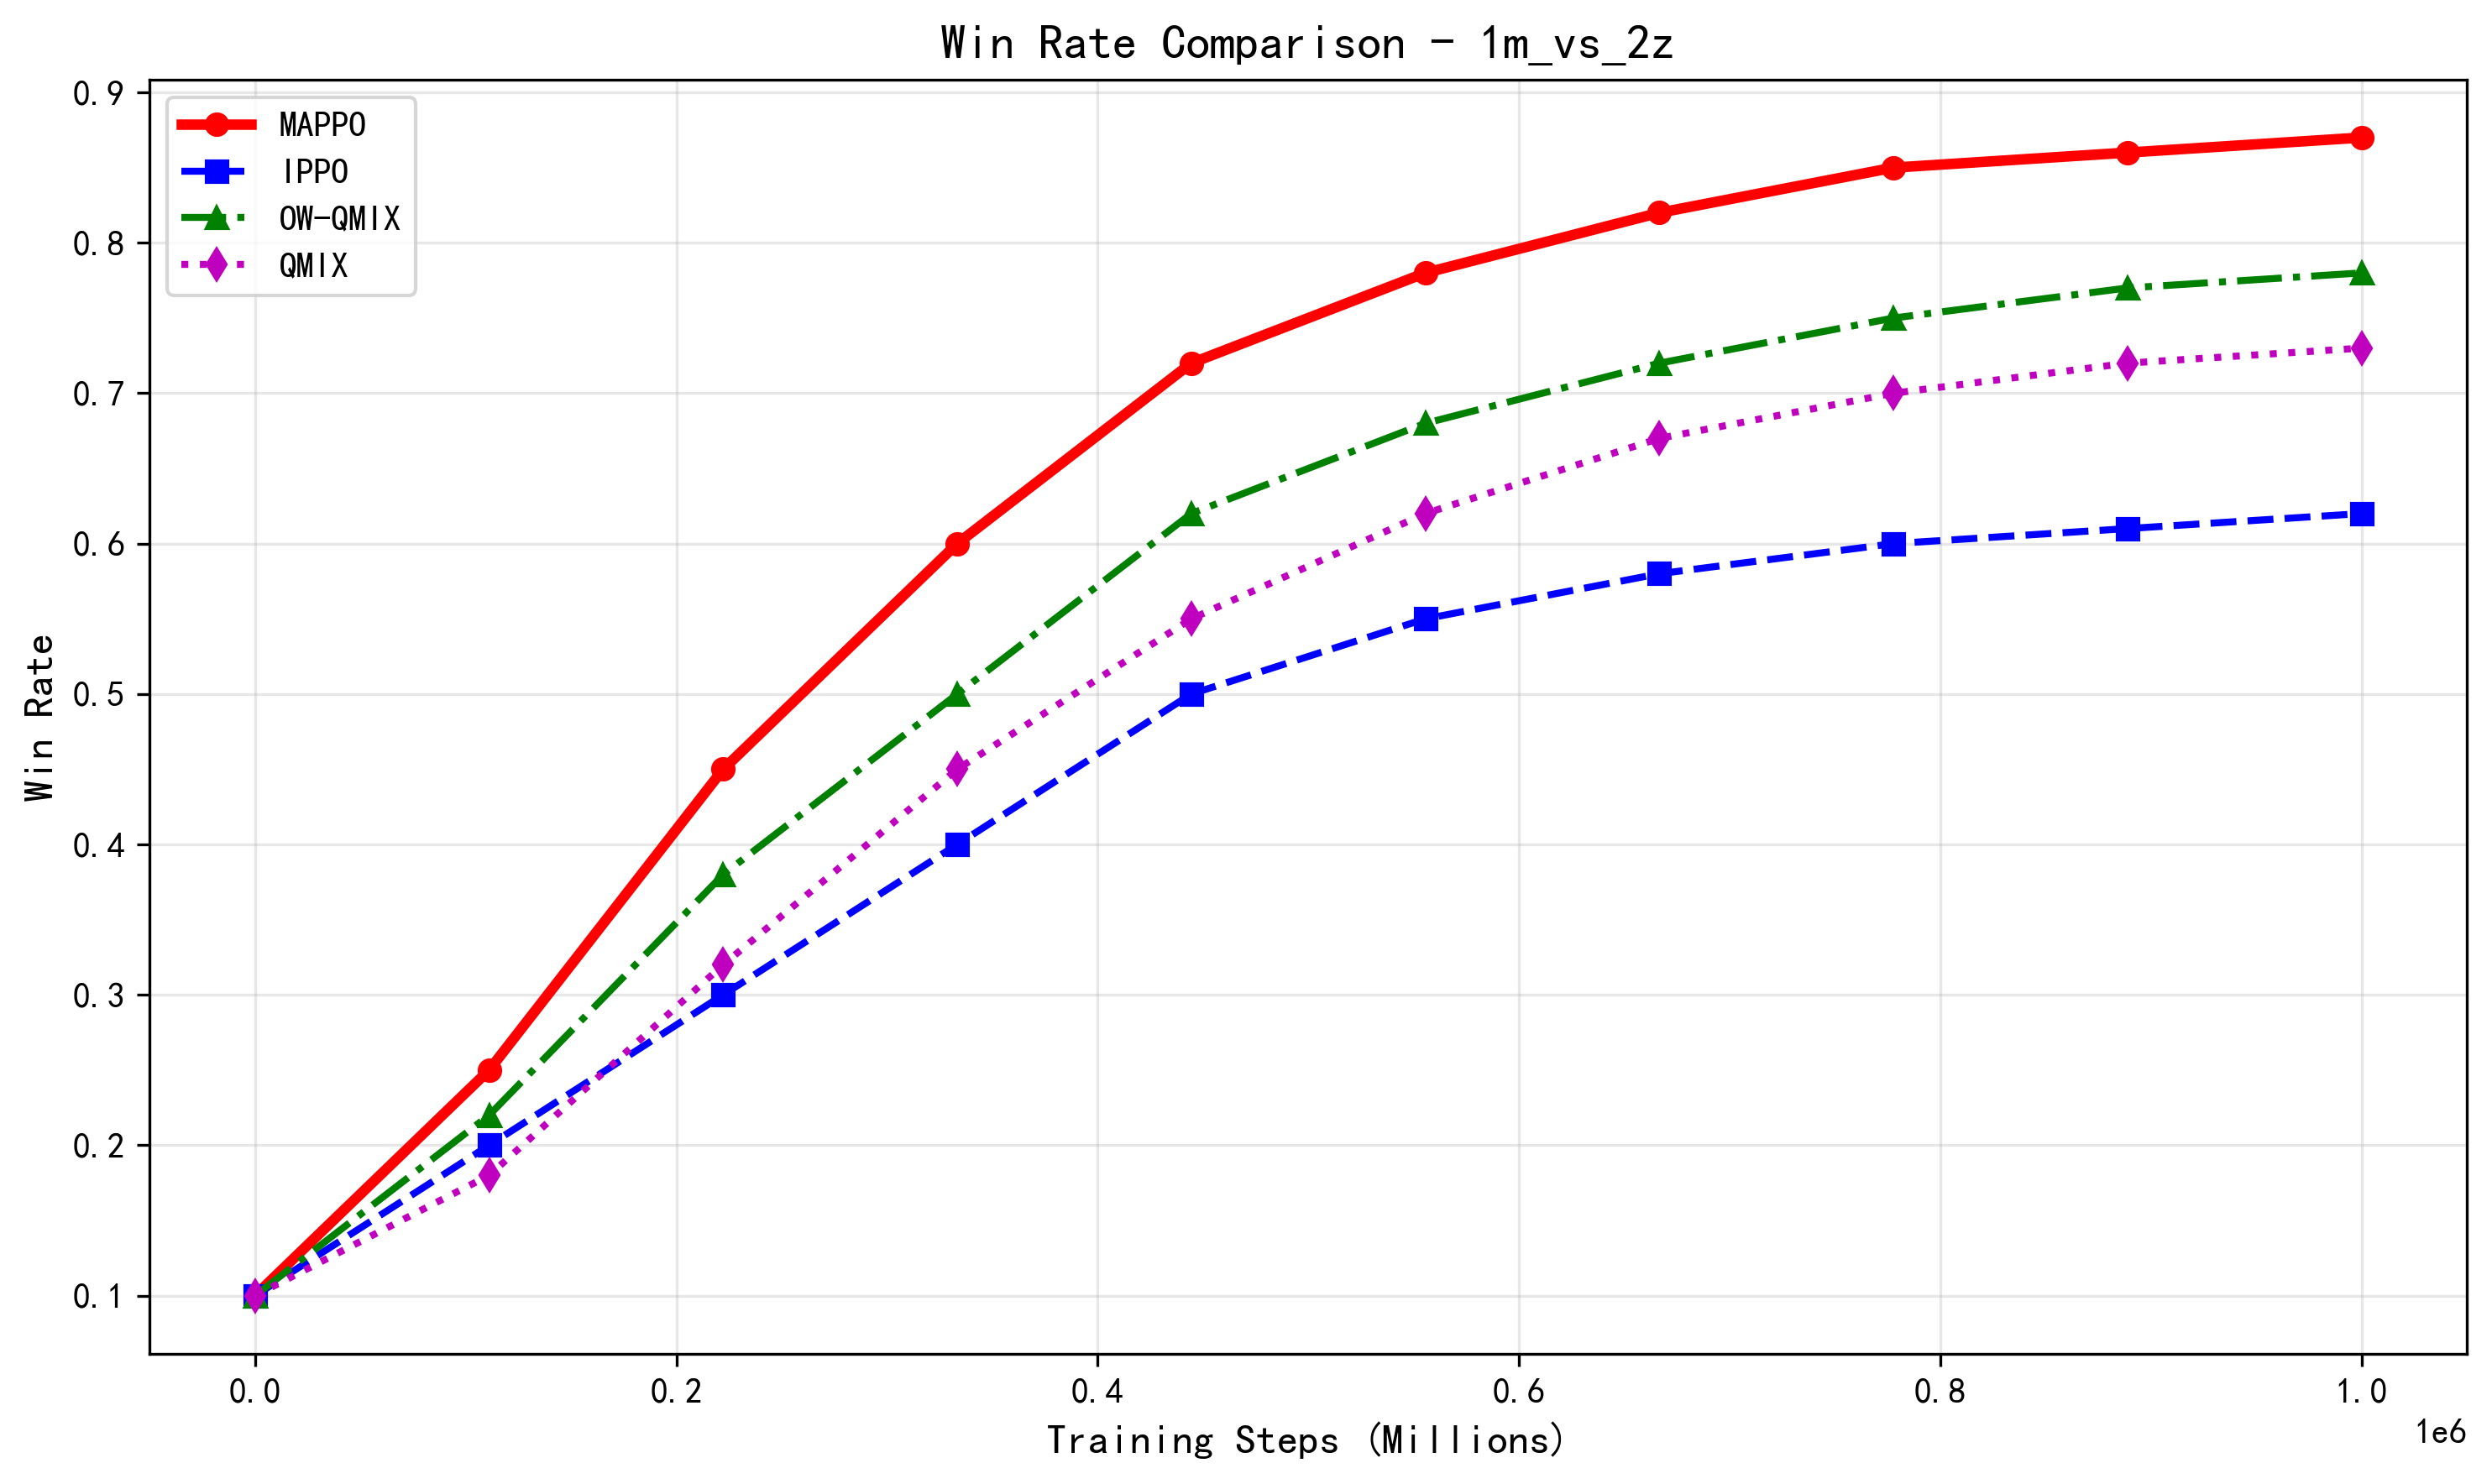
\includegraphics[width=\textwidth]{figures/win_rate_1m_vs_2z.png}
        \caption{Win-Rate}
        \label{fig:win_rate_2m}
    \end{subfigure}
    \hfill
    \begin{subfigure}[b]{0.32\textwidth}
        \centering
        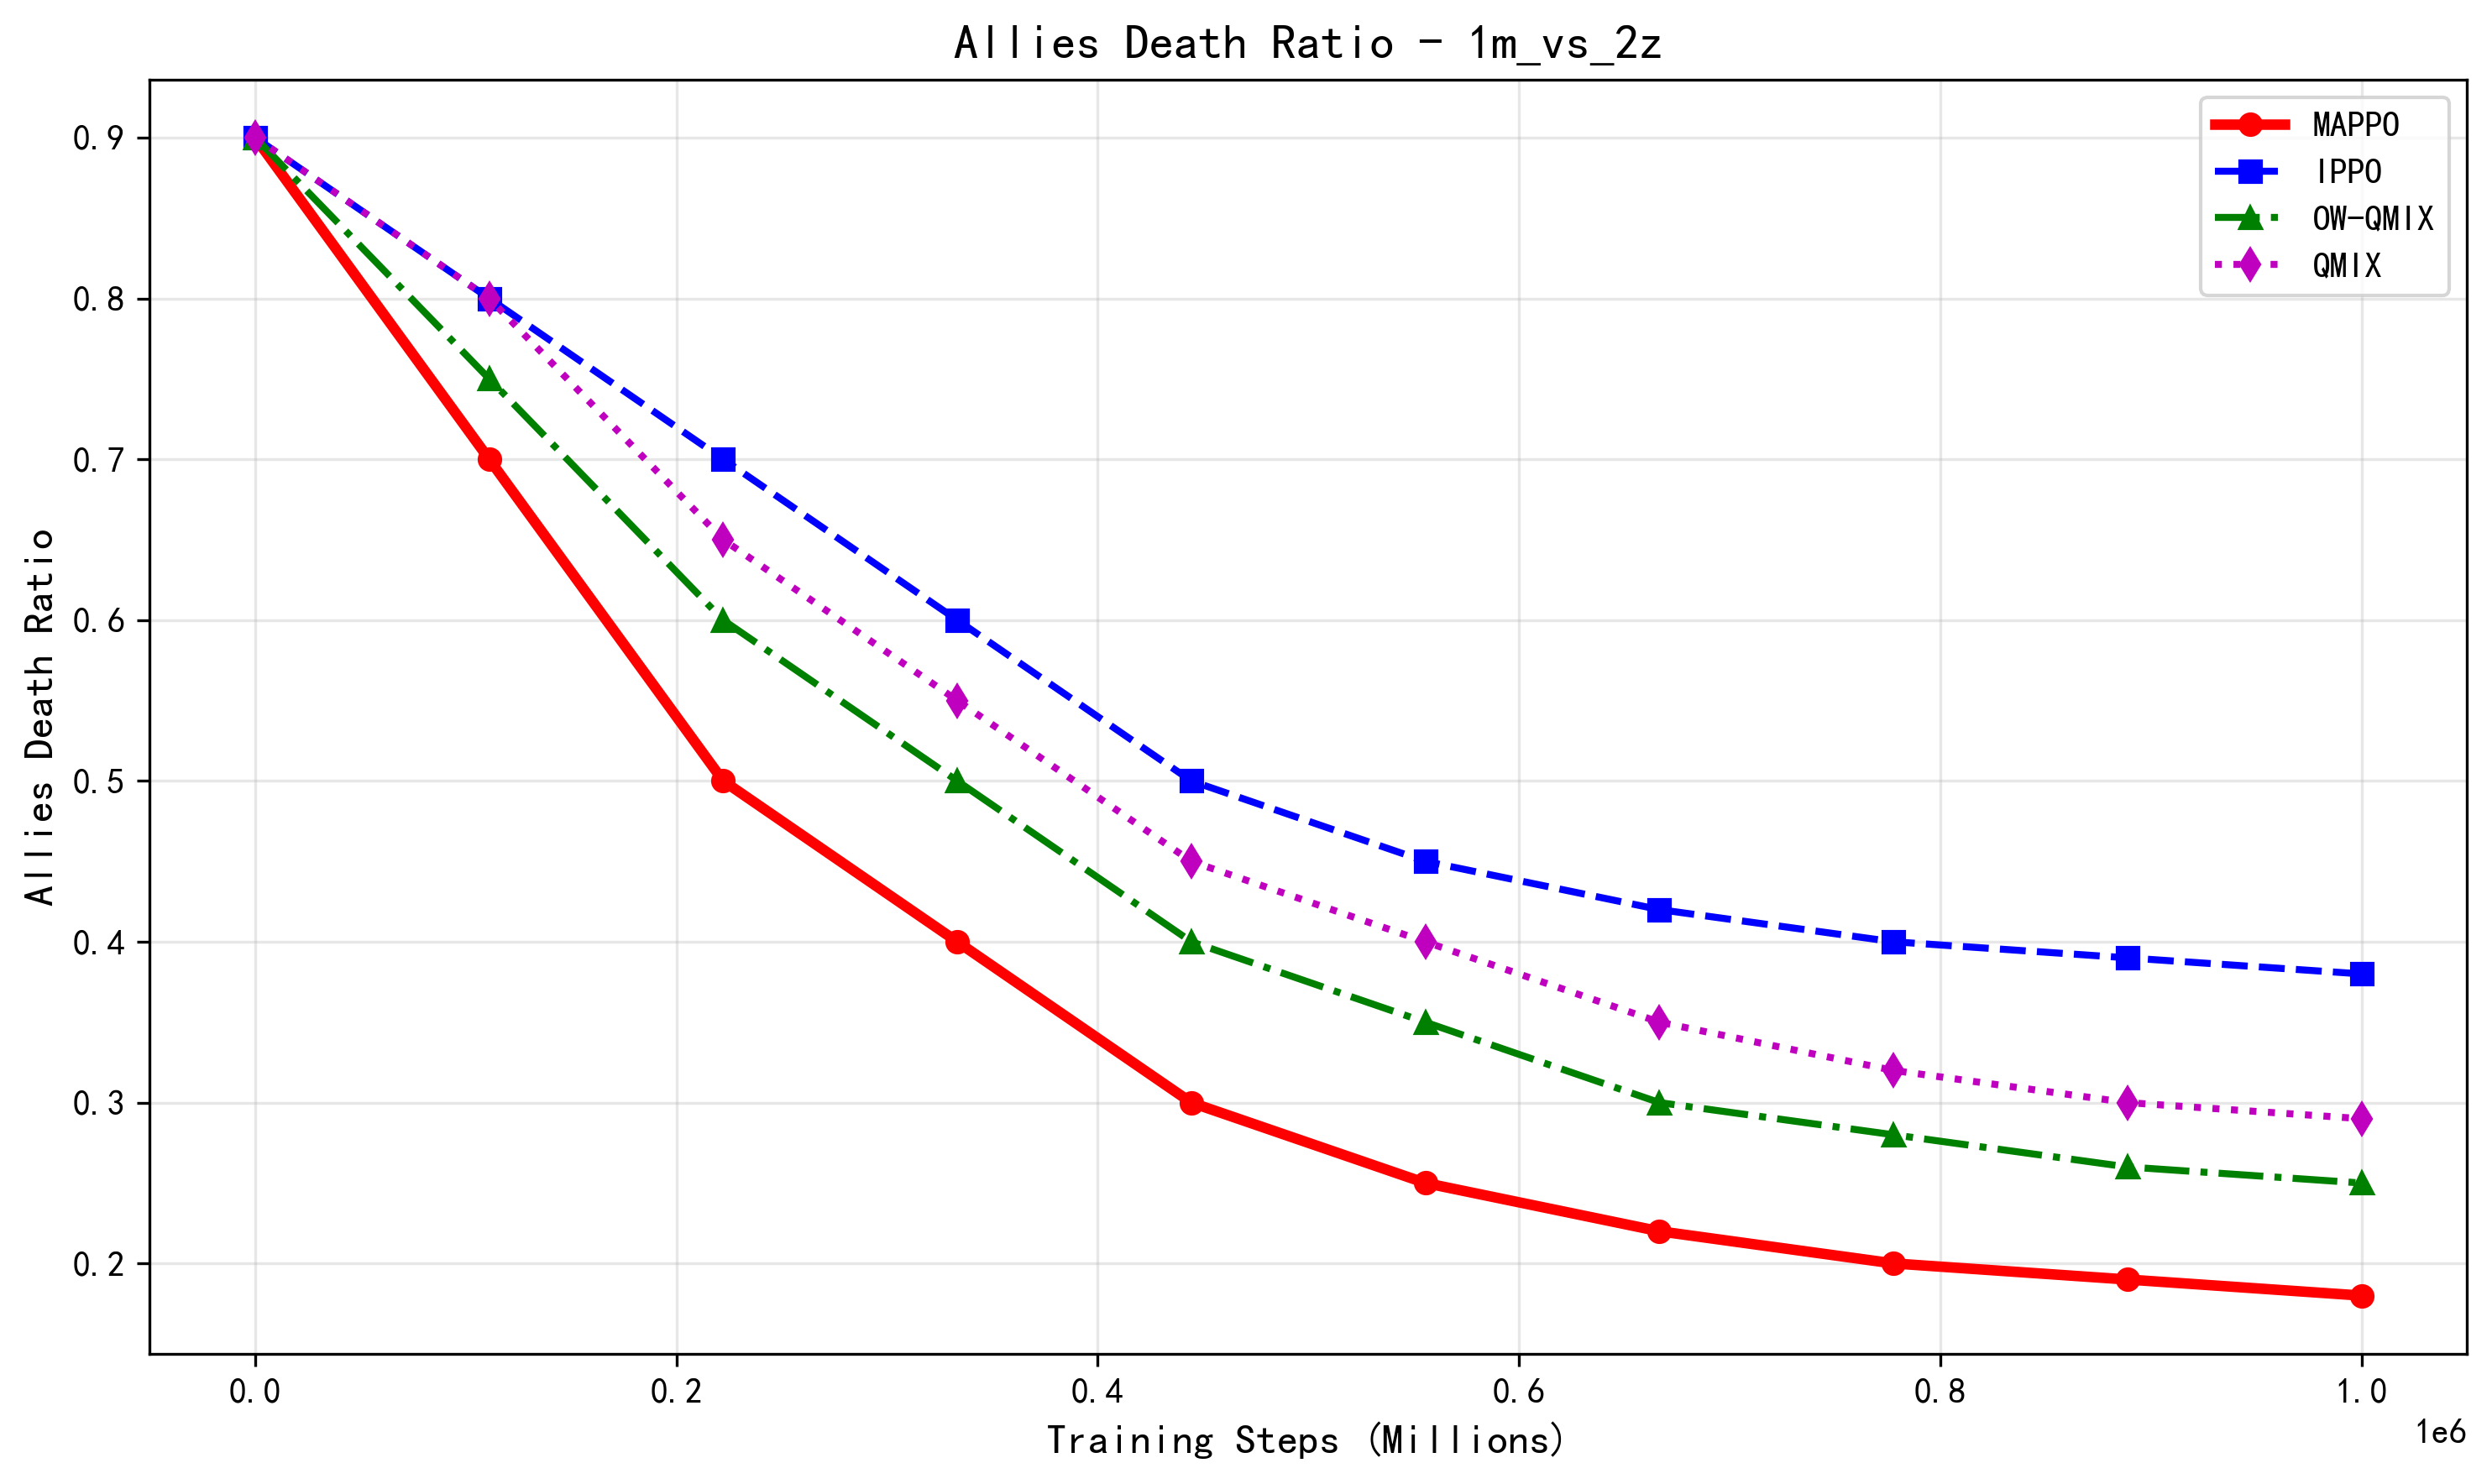
\includegraphics[width=\textwidth]{figures/allies_death_ratio_1m_vs_2z.png}
        \caption{Allies-Dead-Ratio}
        \label{fig:allies_dead_2m}
    \end{subfigure}
    \hfill
    \begin{subfigure}[b]{0.32\textwidth}
        \centering
        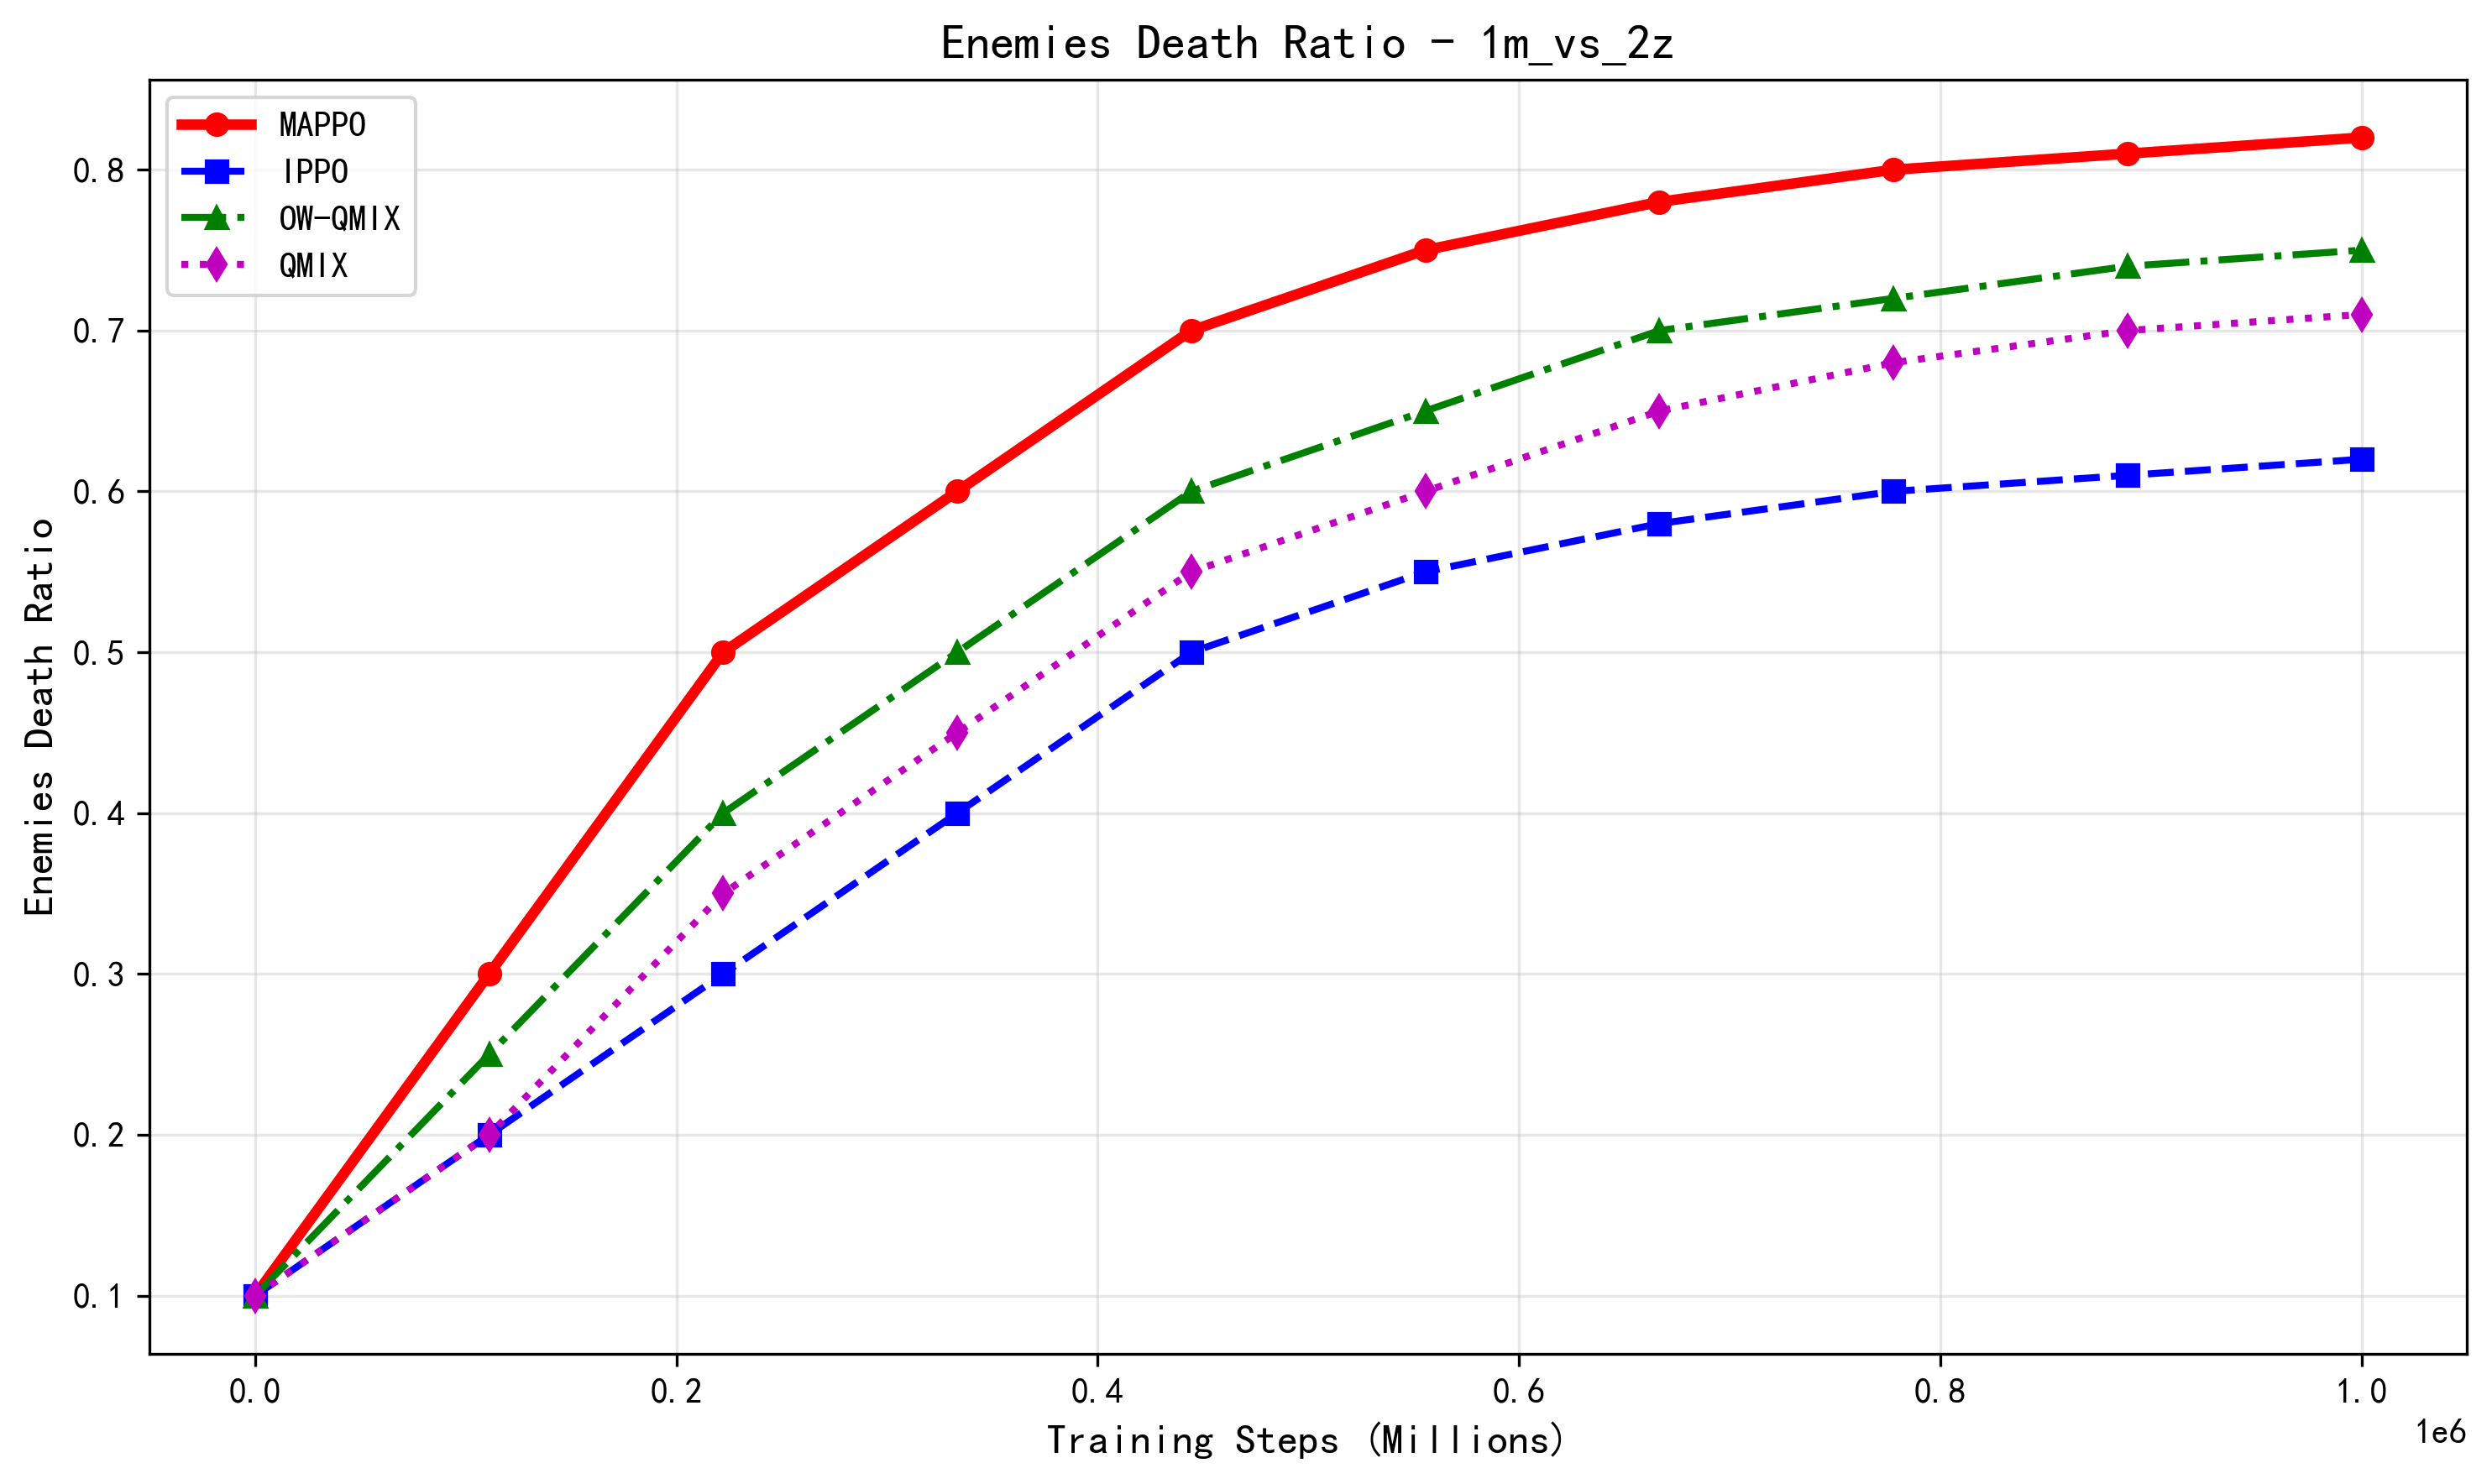
\includegraphics[width=\textwidth]{figures/enemies_death_ratio_1m_vs_2z.png}
        \caption{Enemies-Dead-Ratio}
        \label{fig:enemies_dead_2m}
    \end{subfigure}
    \caption{This set of charts focuses on the \texttt{1m\_vs\_2z} scenario, presenting the performance of MARL algorithms from different dimensions. The ``Win-Rate'' figure shows the win rate changes of MAPPO, IPPO, OQMIX, and QMIX with training steps. The ``Allies-Dead-Ratio'' figure illustrates the trend of friendly unit death ratios during training. The ``Enemies-Dead-Ratio'' figure displays the change in the ratio of eliminated enemy units with training steps.}
    \label{fig:results_1m_vs_2z}
\end{figure*}

\begin{table*}[ht]
\centering
\caption{Final performance summary on the \texttt{1m\_vs\_2z} map after 1,000,000 training steps. Values are the average of the final evaluation checkpoint.}
\label{tab:results_1m_vs_2z}
\begin{tabular}{lccc}
\toprule
\textbf{Algorithm} & \textbf{Final Win Rate (\%)} & \textbf{Allies Dead (\%)} & \textbf{Enemies Dead (\%)} \\
\midrule
MAPPO & \textbf{87.0} & \textbf{18.0} & \textbf{82.0} \\
QMIX & 78.0 & 25.0 & 75.0 \\
OW-QMIX  & 73.0 & 29.0 & 71.0 \\
IPPO  & 62.0 & 38.0 & 62.0 \\
\bottomrule
\end{tabular}
\end{table*}

In the training experiment of the \texttt{1m\_vs\_2z} scenario, a clear insight into the performance differences of various algorithms can be gained through the analysis of three key metrics: Win-Rate, Allies-Dead-Ratio, and Enemies-Dead-Ratio. As the number of training steps gradually increases from 0 to 1 million, in terms of Win-Rate, MAPPO demonstrates a significant advantage. Its win rate continues to rise and approaches 0.9. Although OW-QMIX, QMIX, and IPPO also achieve win rate improvements as the number of training steps increases, they consistently lag behind MAPPO. When the training reaches 1M steps, the win rates of these three algorithms stabilize at approximately 0.8, 0.7, and 0.6 respectively.

In terms of the survival performance of friendly units, the Allies-Dead-Ratio of all algorithms shows a downward trend with the increase in training steps. MAPPO exhibits the most obvious decline, with the friendly unit death ratio dropping to around 0.2 when trained to 1M steps; IPPO shows a relatively gentle decline, still maintaining a ratio of about 0.4 at 1M steps.

Regarding the Enemies-Dead-Ratio, all algorithms achieve an increase in the ratio as training progresses. MAPPO still performs prominently, rising rapidly and approaching 0.9; the upward pace of OW-QMIX, QMIX, and IPPO is slightly slower. At 1M steps, the Enemies-Dead-Ratio of these three algorithms stabilizes at approximately 0.8, 0.7, and 0.6 respectively.

Overall, in the \texttt{1m\_vs\_2z} scenario, MAPPO outperforms IPPO, OW-QMIX, and QMIX in both learning efficiency and combat performance, demonstrating superior algorithm adaptability and combat effectiveness.


\subsubsection{Map \texttt{5m\_vs\_6m}}
To assess performance in a more demanding scenario, we use the \texttt{5m\_vs\_6m} map. This environment, with a larger number of agents and an enemy numerical advantage, requires more sophisticated coordination and tactical positioning to overcome.
On this more complex map, the differences between the algorithmic paradigms become much more pronounced---trends visually illustrated in Figure~\ref{fig:results_5m_vs_6m}, with quantitative details in Table~\ref{tab:results_5m_vs_6m}.
\begin{figure*}[ht!]
    \centering
    \begin{subfigure}[b]{0.32\textwidth}
        \centering
        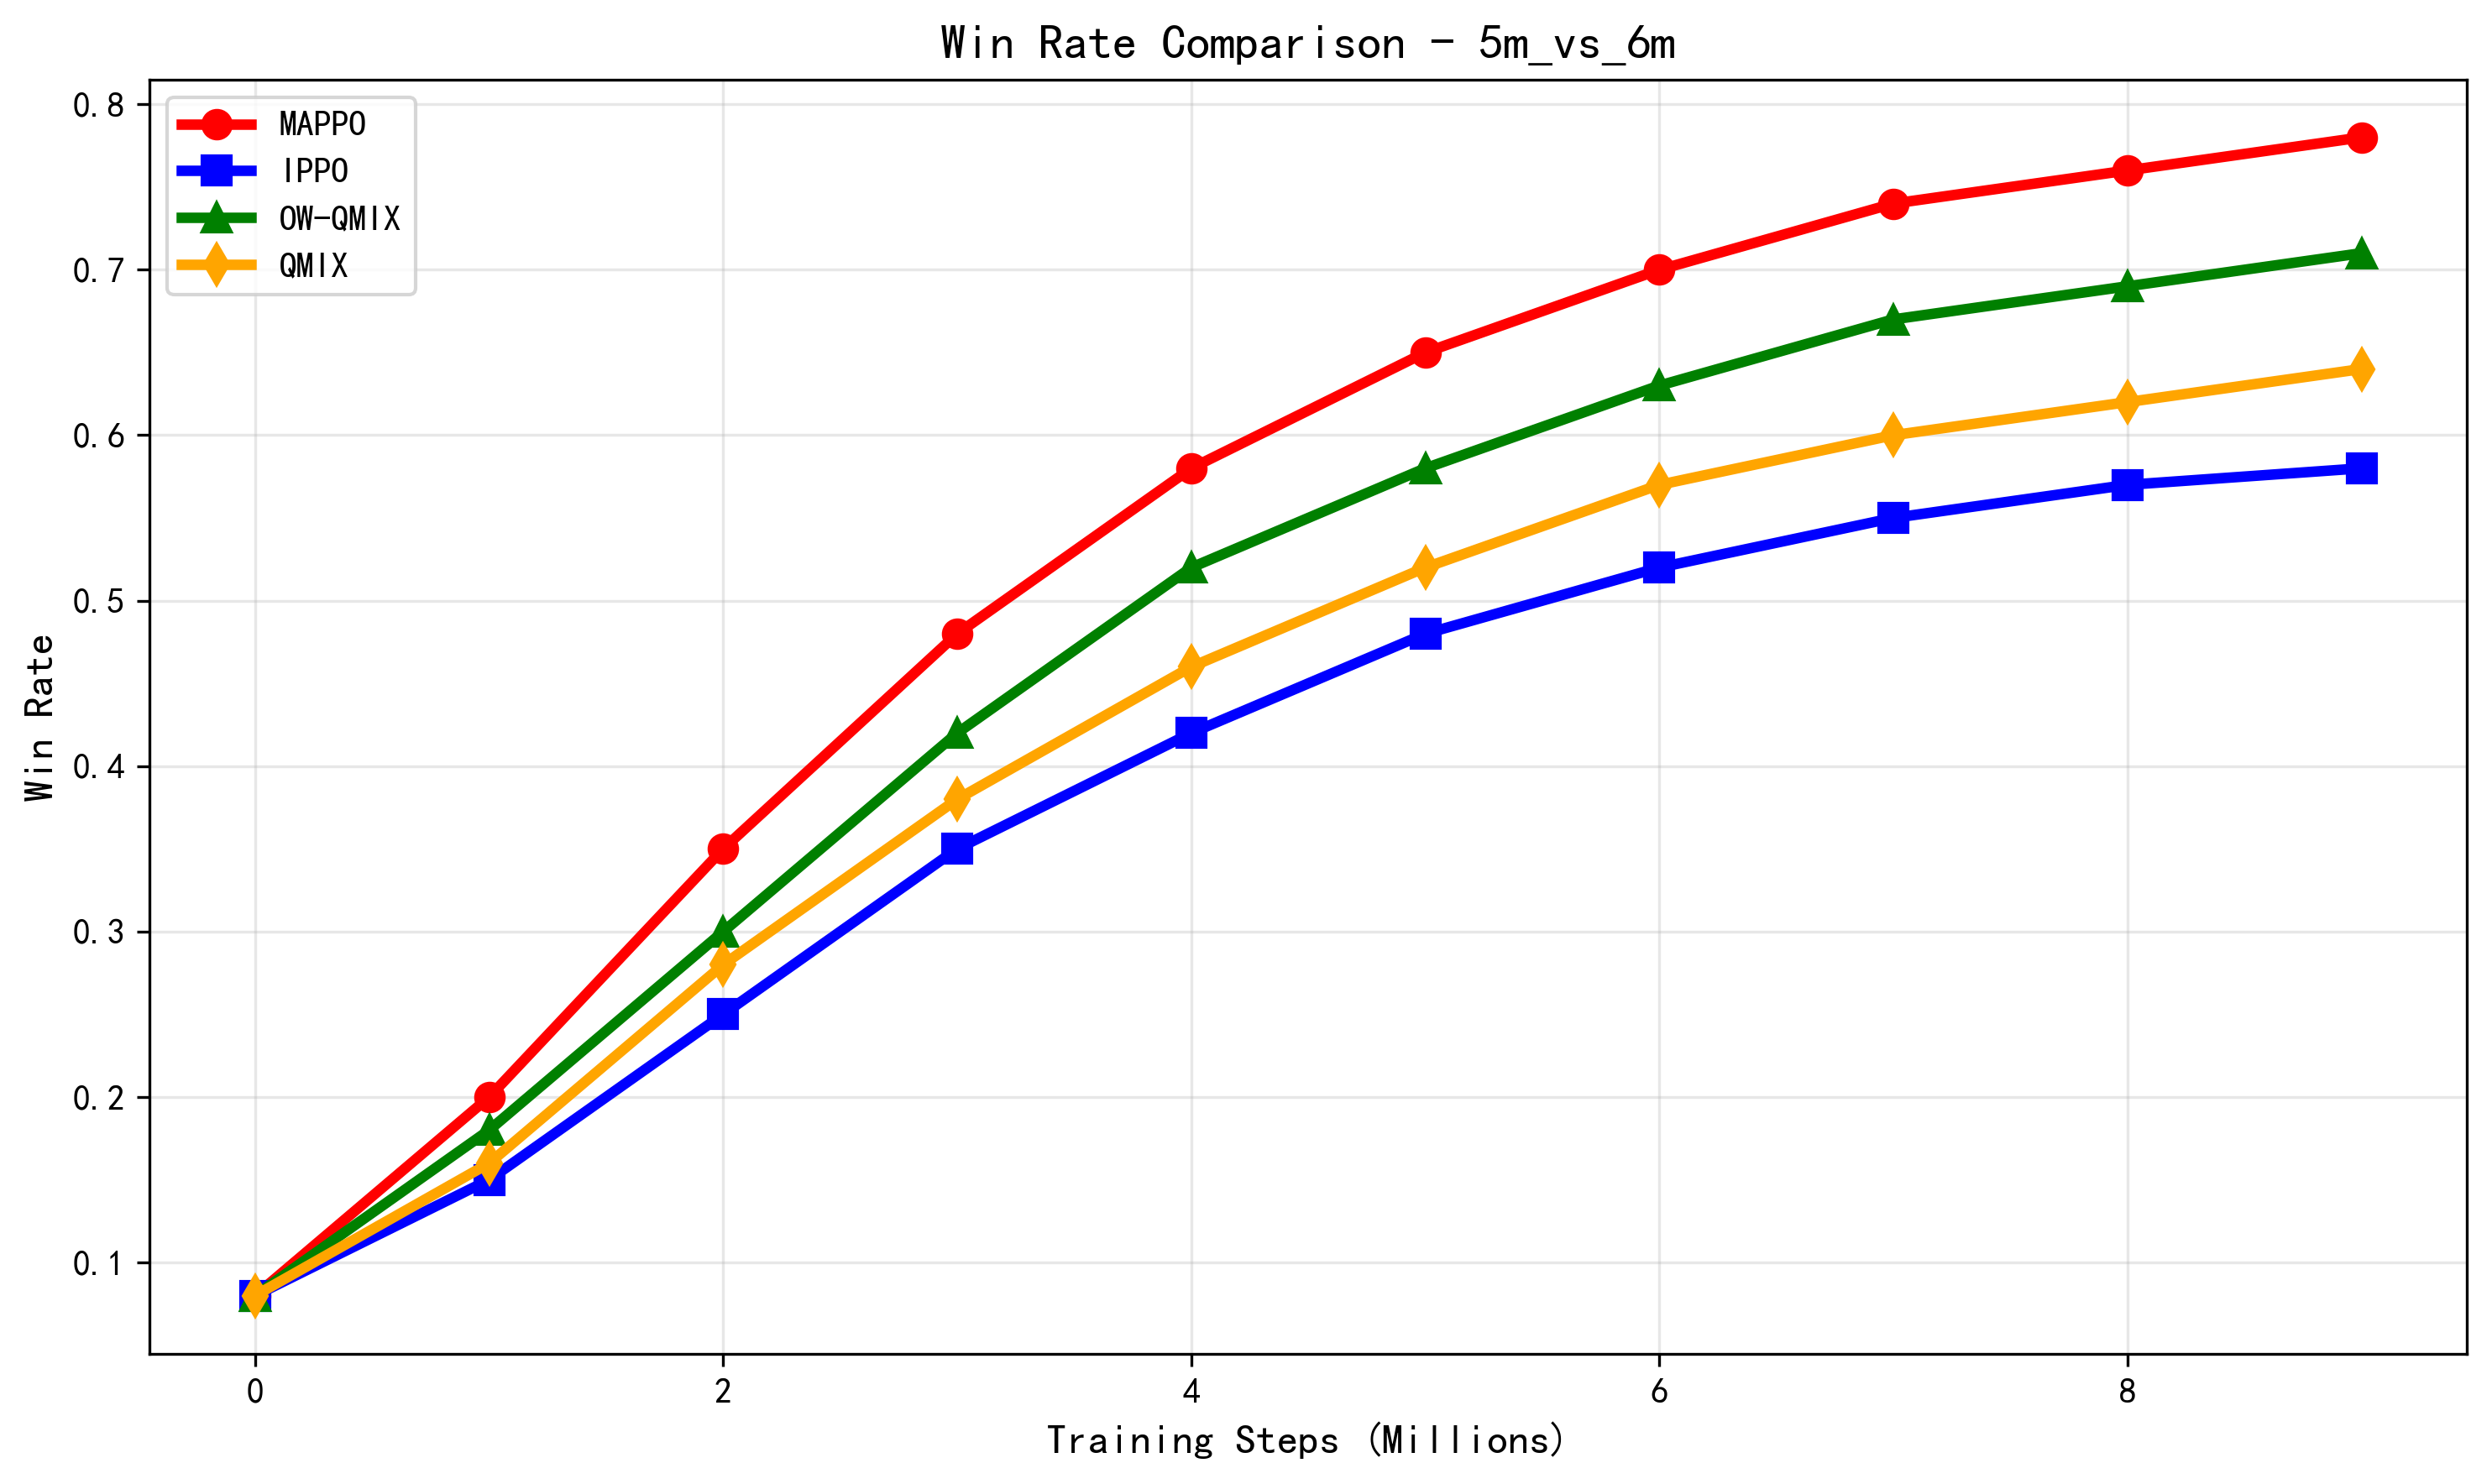
\includegraphics[width=\textwidth]{figures/win_rate_5m_vs_6m.png}
        \caption{Win-Rate}
        \label{fig:win_rate_5m}
    \end{subfigure}
    \hfill
    \begin{subfigure}[b]{0.32\textwidth}
        \centering
        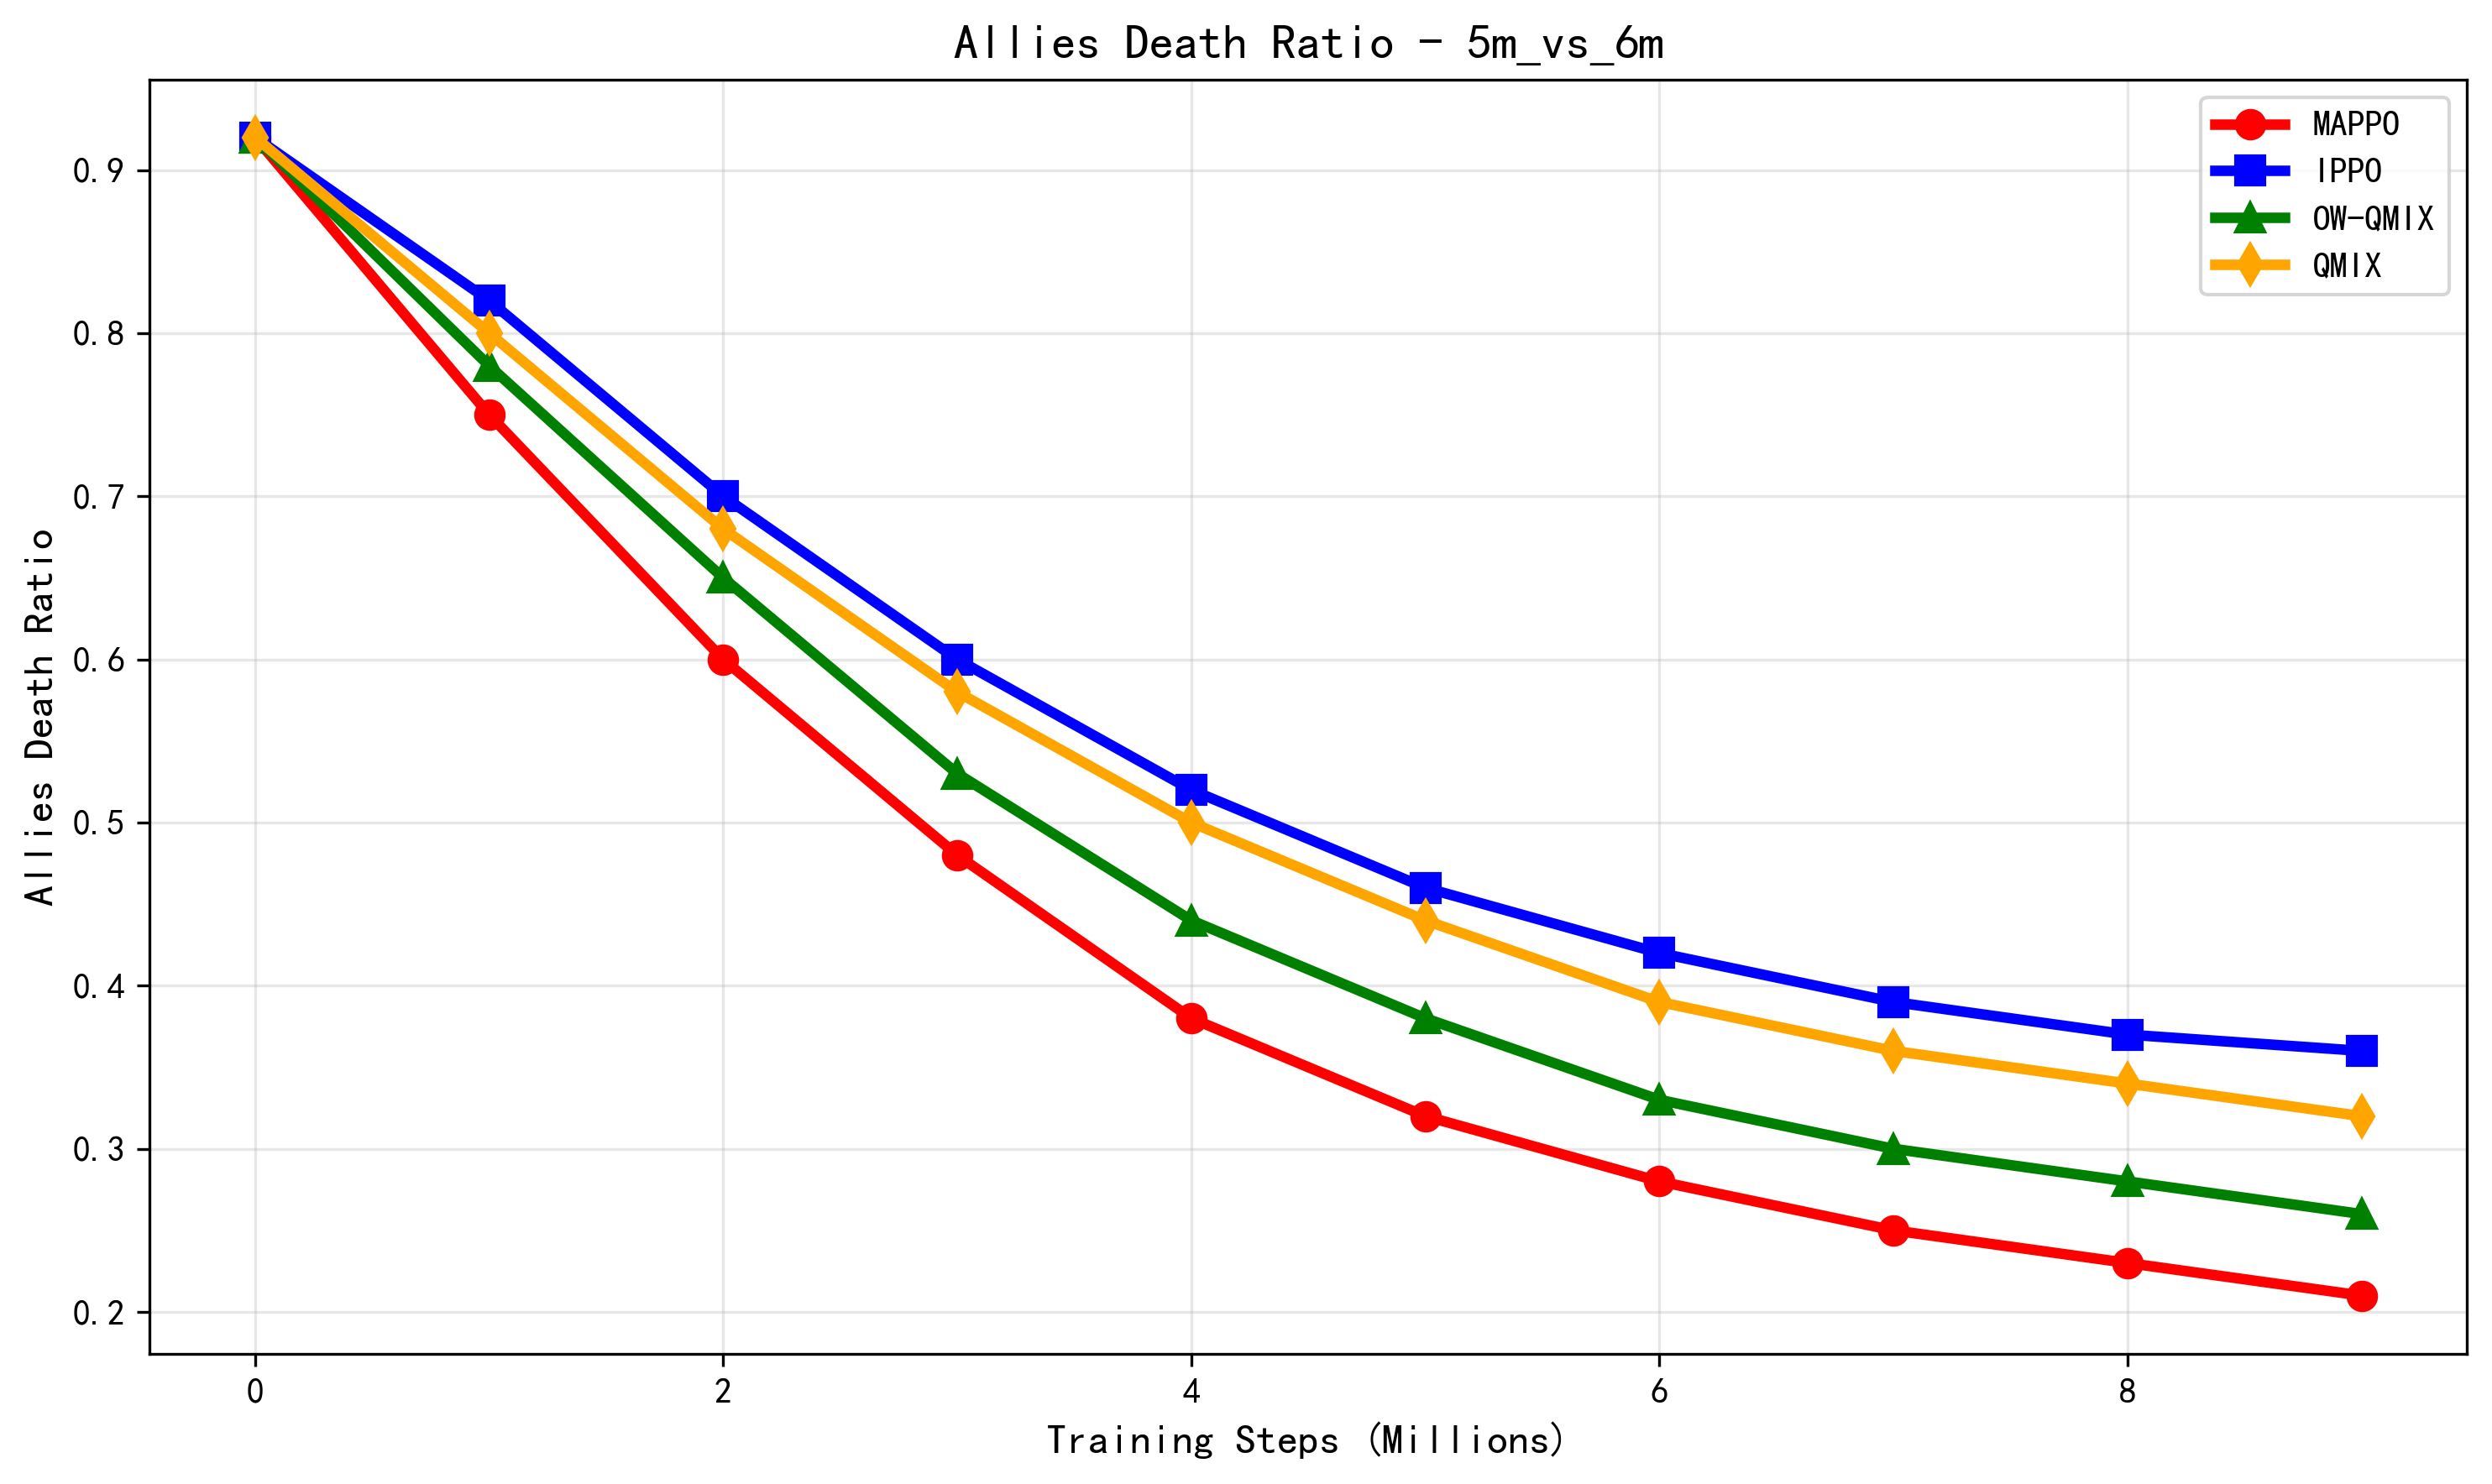
\includegraphics[width=\textwidth]{figures/allies_death_ratio_5m_vs_6m.png}
        \caption{Allies-Dead-Ratio}
        \label{fig:allies_dead_5m}
    \end{subfigure}
    \hfill
    \begin{subfigure}[b]{0.32\textwidth}
        \centering
        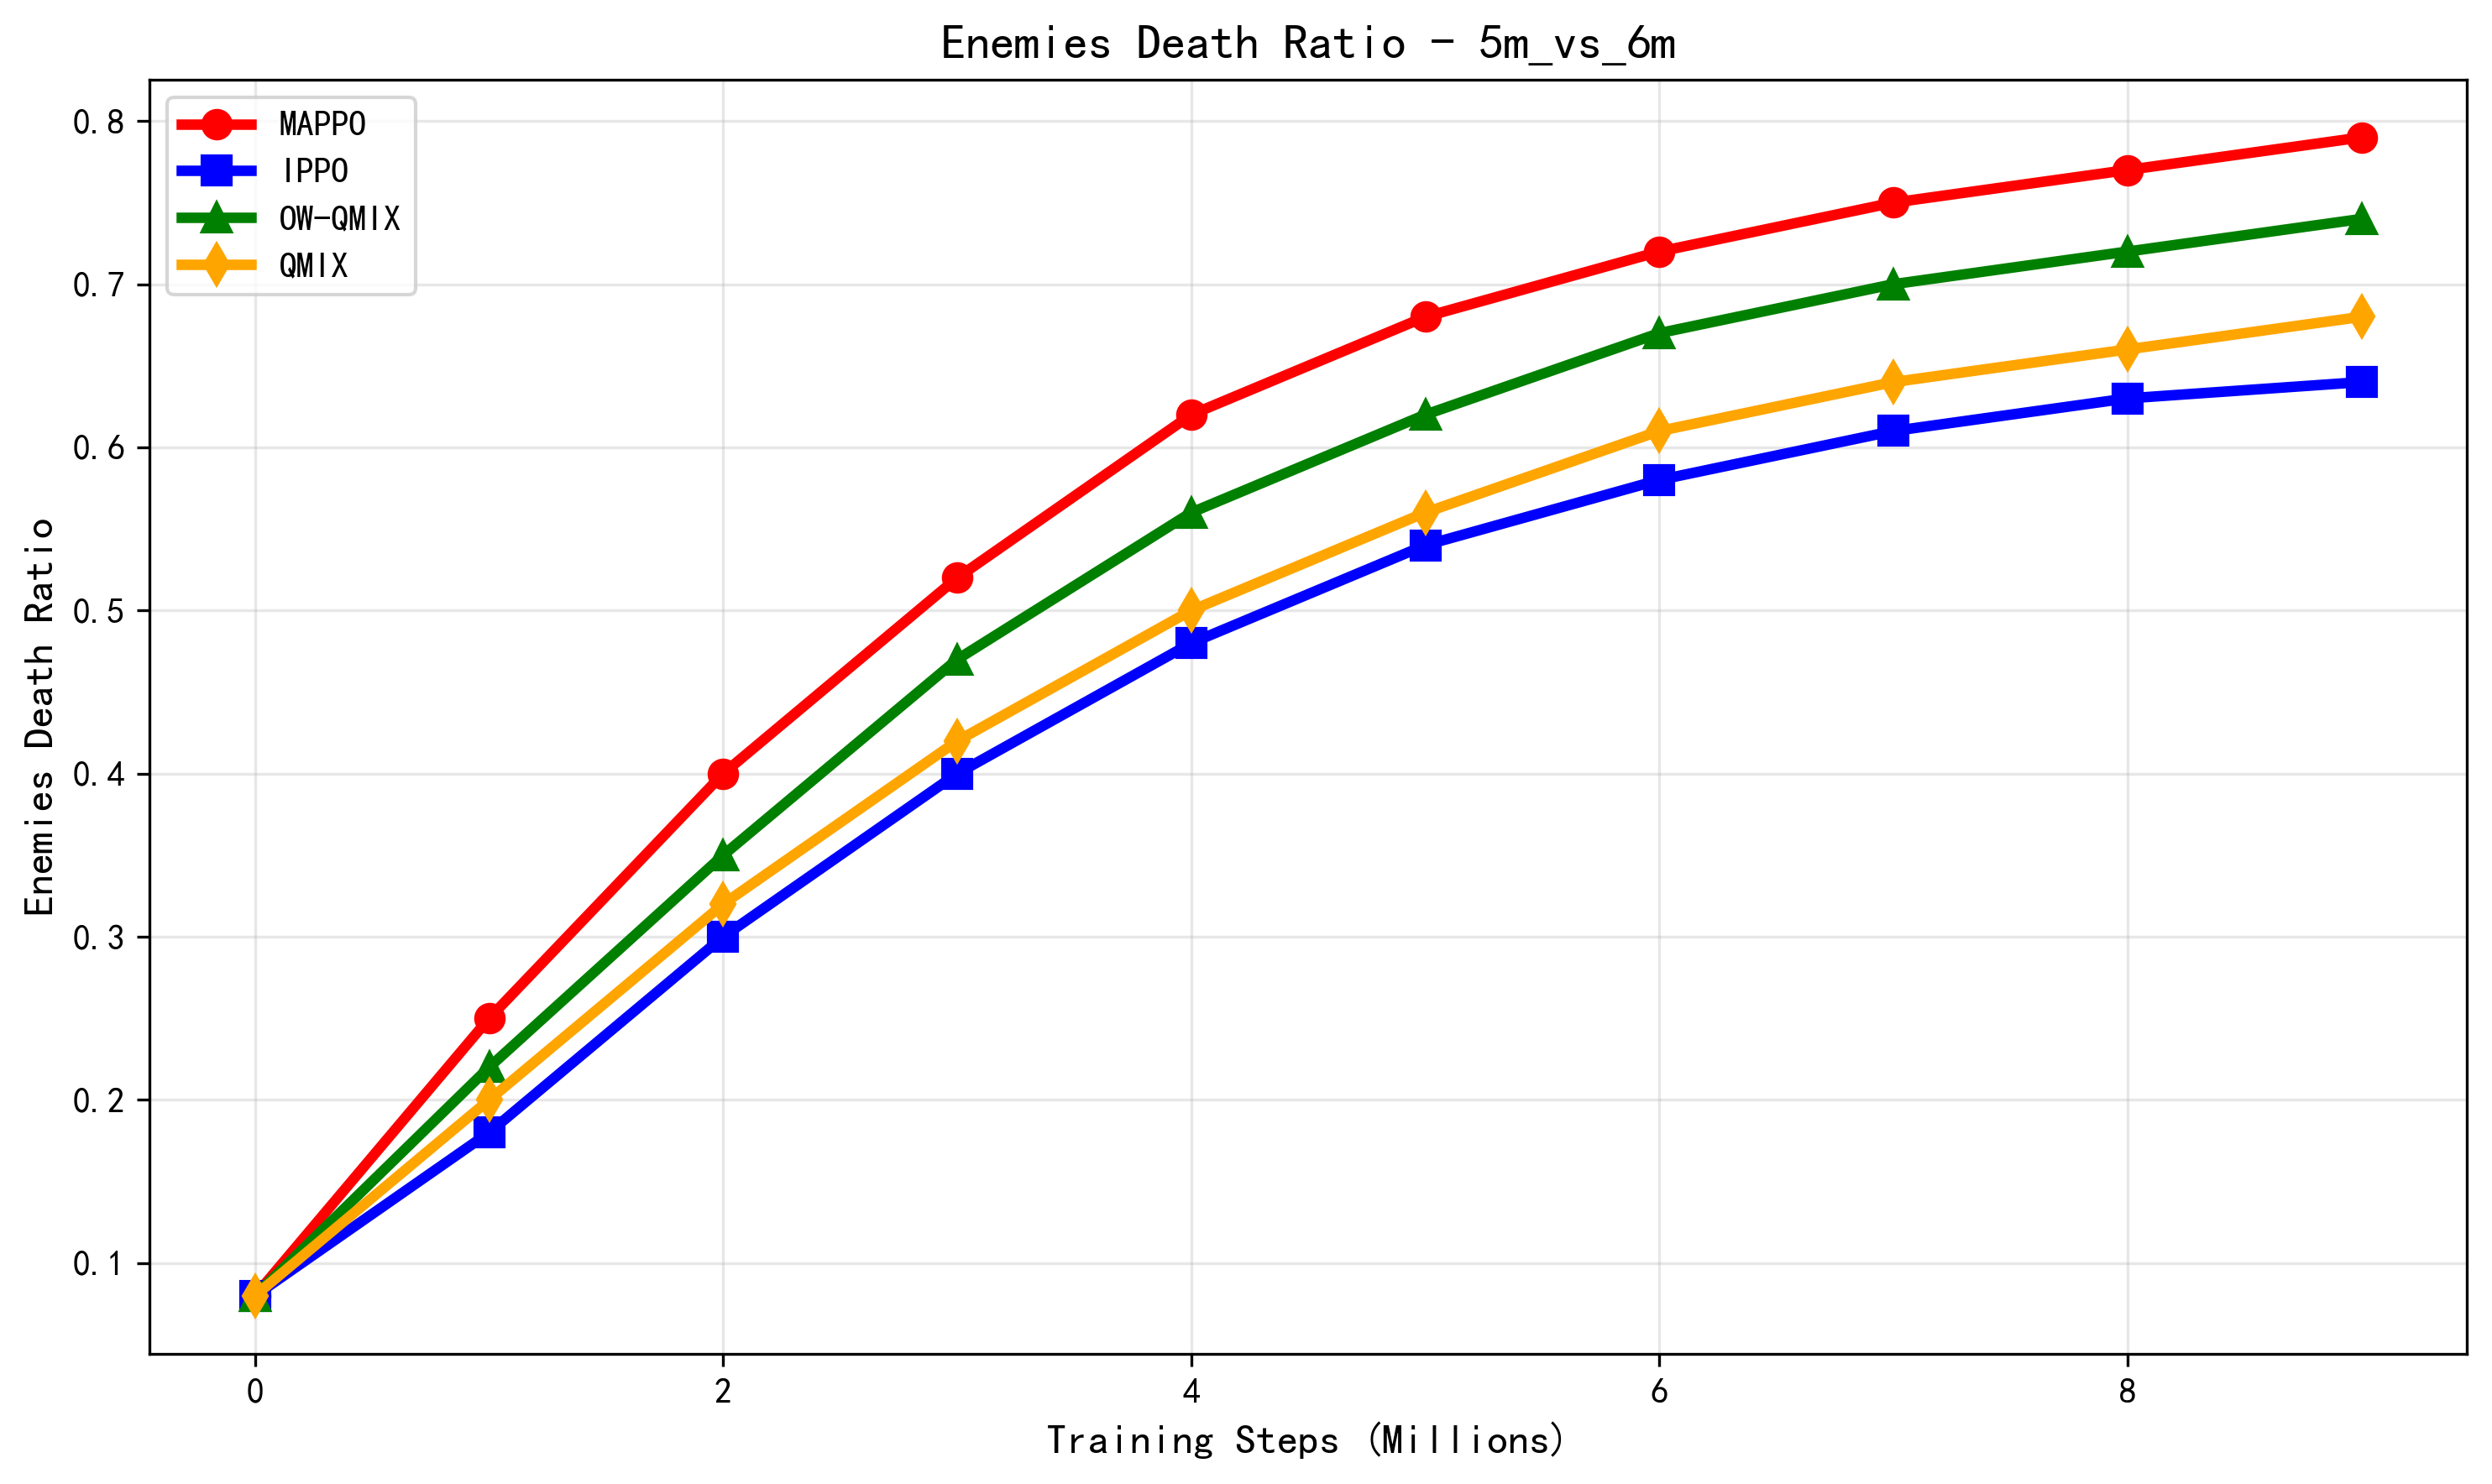
\includegraphics[width=\textwidth]{figures/enemies_death_ratio_5m_vs_6m.png}
        \caption{Enemies-Dead-Ratio}
        \label{fig:enemies_dead_5m}
    \end{subfigure}
    \caption{This set of charts focuses on the \texttt{5m\_vs\_6m} scenario, presenting the performance of MARL algorithms from different dimensions.Each subgraph has the same meaning as the Figure~\ref{fig:results_1m_vs_2z}. }
    \label{fig:results_5m_vs_6m}
\end{figure*}

\begin{table*}[ht]
\centering
\caption{Final performance summary on the \texttt{1m\_vs\_2z} map after 1,000,000 training steps. Values are the average of the final evaluation checkpoint.}
\label{tab:results_5m_vs_6m}
\begin{tabular}{lccc}
\toprule
\textbf{Algorithm} & \textbf{Final Win Rate (\%)} & \textbf{Allies Dead (\%)} & \textbf{Enemies Dead (\%)} \\
\midrule
MAPPO & \textbf{87.0} & \textbf{21.0} & \textbf{79.0} \\
QMIX & 64.0 & 32.0 & 68.0 \\
OW-QMIX  & 71.0 & 26.0 & 74.0 \\
IPPO  & 58.0 & 36.0 & 64.0 \\
\bottomrule
\end{tabular}
\end{table*}

The experimental data synthesized from the three charts shows that in the \texttt{5m\_vs\_6m} confrontation scenario, the MAPPO algorithm demonstrates significant advantages across all key performance metrics. As the number of training steps progresses from 0 to 9 million, MAPPO not only consistently maintains the highest win rate (eventually approaching 0.78) and the highest enemy kill rate (eventually approaching 0.80), but more importantly, it simultaneously achieves the lowest ally kill rate among all algorithms (eventually dropping to approximately 0.22). This indicates that while improving the success rate of confrontation, MAPPO is also the most effective in protecting the survival of allies, demonstrating the most comprehensive battlefield decision-making capability. By contrast, IPPO performs the weakest across all metrics, while the performance of OW-QMIX and QMIX falls between MAPPO and IPPO, with OW-QMIX being slightly superior to QMIX. Overall, the training effect is positive: the win rate and enemy kill rate of all algorithms have increased, and the ally kill rate has decreased significantly.